\section{Mapping}
\label{sec:mapping}
{\em Mapping definitions} describe how to map a single molecule from an atomistic to a coarse-grained representation. A mapping definition has to be specified only once per molecule. The file contains sections for coarse-grained beads, bonded interactions in the coarse grained scheme as well as mapping matrices. If a system contains several molecule types, it has to be enssured that molecule names are set properly. The mapping files should be specified in a list separated by ; (e.g. "protein.xml;solvent.xml"). The \xmlopt{ident} tag in the mapping definition must match the name of the molecule in the reference system.

The mapping file has similar entries as a topology, but contains additional information for mapping are present. In the topology section, coarse grained beads and bonded interactions are defined. Each coarse grained bead has a name, type and mapping entry, as well as a list of atoms which are mapped to it. The name must be unique within the mapping file. Type defines the type of the bead. The \xmlopt{mapping} tag defines which mapping scheme is used from the mapping section in the file. Type and mapping can be different since the number of atoms for the same bead type may differ, e.g. at chain ends for saturating hydrogen atoms.

In the \xmlopt{mapping} section, the mapping operator is defined. Currently this includes only weights for a linear mapping scheme.

A complete reference for mapping file definitions can be found in ref.~\ref{sec:ref_mapping}. To map from atomistic to a reference system, \textbf{csg\_map} can be used:
\begin{verbatim}
  csg_map --top topol.tpr --trj traj.trr --cg "protein.xml;solvent.xml" --out cg.gro
\end{verbatim}

To create an coarse-grained topology based on the mapping scheme, see \textbf{csg\_gmxtopol}.

\subsection{Example - mapping file for propane}
\begin{figure}[ht]
  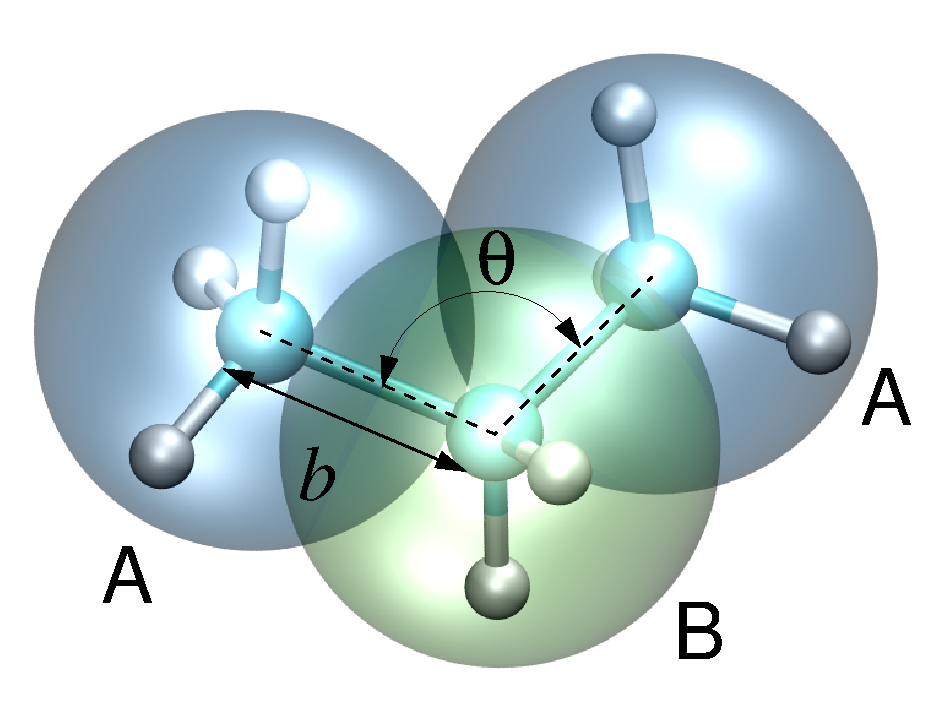
\includegraphics[width=0.4\textwidth]{functionality/fig/propane.eps}
  \caption{Mapping for propane}
\end{figure}

\lstinputlisting{functionality/propane.xml}
